%\NeedsTeXFormat{LaTeX2e}[1995/01/01]
\documentclass[10pt,twocolumn]{article}
\usepackage{latex8}
\usepackage{times}
% Predefined packages
%
%\usepackage[english]{babel}
%\usepackage{a4wide}
\usepackage{epsfig}
%\usepackage{psfig}
\usepackage{bigbox}
\usepackage{graphicx}
\usepackage{float}
\usepackage{url}
\usepackage{xspace}
\usepackage[T1]{fontenc}
\usepackage[latin1]{inputenc}
%\usepackage{doublespace}

\newcommand{\audio}{conference call\xspace}
%\floatplacement{figure}{H}
\pagestyle{empty}

%\usepackage{hrefpdf}

\begin{document}

\title{A Service-Component Testing Method and a Suitable CORBA Architecture}
\author{Ana Cavalli, Bruno Defude, Christian Rinderknecht, Fatiha Za�di\\
Institut National des T�l�communications\\
9 rue Charles Fourier\\
F-91011 �vry Cedex\\
\{Ana.Cavalli, Bruno.Defude, Christian.Rinderknecht,
Fatiha.Zaidi\}@int-evry.fr}

\maketitle
\thispagestyle{empty}

\begin{abstract}
This paper presents a method for service-component testing and a
suitable CORBA test architecture. This test environment allows the
service validation from its components and is a close step towards the
execution of the obtained tests on a CORBA environment. Two aspects
are relevant: the test of components and the test architecture. The
testing method for components is new: it is based on the generation of
partial graphs and avoids the combinatorial explosion of number of
states of the global system. The test architecture on a CORBA platform
is also new, since there are few works on testing based on these
environments. As an application we present a case study on a real
\audio service.\\ {\bf Keywords} Components testing, test generation,
test architecture, CORBA
\end{abstract}

%\submitted[March 1st, 2000]{ICNP}{1}

%%-*-latex-*-

\section{Introduction}

The telecommunication operators are facing the dramatic growth of new
services that utilize the telephonic network but also mix voice
transmission with image and sound transmission. The inherent
difficulty of this kind of services lies on their fast and reliable
integration, in order to satisfy the users' requirements.

The Intelligent Network (IN) has been the first attempt to solve this
sort of problems and, in the meanwhile, some others architectures have
been proposed, like TINA, in order to cope efficiently with the design
and the implementation of new services. These latter must meet the
users' expectations and be definitely reliable. With this aim, after
the design phase, the services should be validated and tested in order
to guarantee that the proposed implementations comply with the
requirements. Moreover, because of modularity and reusability
constraints, these services are to be defined from base components
which may further be combined and reused.
%\begin{figure}[!ht]
%\begin{center}
%\begin{bigbox}
%\epsfxsize=8cm
%\epsfbox{test_process.eps}
%\end{bigbox}
%\caption{Process of test production}
%\label{test_process}
%\end{center}
%\end{figure}

In this paper we present a method for service-component testing and a
Corba test architecture. To illustrate the application of the method we
present a case study: a \audio service. 
%The general architecture of this test environment is shown at
%figure~\ref{test_process}. 
Our input is an SDL
model of the service we want to test. Starting from this model, we
generate a test sequence by using the component test algorithm,
Hit-or-Jump. This sequence is built from the SDL model and is
thus expressed in terms of SDL entities. The values associated to
the exchanged signals have types represented within SDL. In order to
step forward the test execution on a CORBA environment, this sequence
must be transformed to be defined in terms of CORBA objects, and hence
mapped to the IDL language. Last, an execution environment on
a CORBA architecture is proposed.

The contribution of this work lies on the methods definition for the
service-component testing and the test execution architecture on a
CORBA environment. At the CFIP99~\cite{cfip99}, we have presented yet
a method for the embedded testing, but this method was based upon the
generation of the whole accessibility graph of the system under test.
The method presented here is new, it is based on the production of
partial accessibility graphs and in this way avoids the combinatorial
explosion of the state number of the global system.

We also present in this work the test execution architecture on a
distributed CORBA environment. We give the principles allowing the
test of a CORBA implementation by combining interactive and purely
observational techniques (also called \emph{passive testing}). This
approach is innovative since, to our knowledge, there exists very few
works on validation and test execution for CORBA environments.

This work was achieved in the CASTOR RNRT French
project~\cite{castor}. The specification of the \audio service was
provided by France Telecom R\&D.

This article is organized as follows. In
section~\ref{generation_de_tests} we give a short overview of the
algorithm used for the derivation of the service-components
tests. Section~\ref{descriptif_specification} presents the case study,
the \audio and its components. Moreover, in this section we 
present the results of the experiments we have made. Then
section~\ref{CORBA} presents a description of the CORBA environment
devoted to test execution, and explains the principles which guided
its design. Last, section~\ref{conclusion} gives the conclusions of
this work.





%%-*-latex-*-

\section{A service-component testing method\label{generation_de_tests}} 

\subsection{Preliminaries}

In this section we present briefly the method used for the generation
of component tests. A more complete presentation can be found
in~\cite{chine}. A comparison with the existing
methods~\cite{bourhfir,IEEE} is presented in~\cite{cfip00}. Some tools
devoted to the embedded testing (or \emph{testing in context}) are
presented in~\cite{testcomposer,groz}.

The aim of the method is to test components in their context, i.e. the
complement of the component in the system, because usually there is
no direct access to the component. The system is defined in terms of
\emph{Communicating Extended Finite-State Machines} (CEFSMs), which
are based upon \emph{Extended Finite-State Machines} (EFSM) defined as
follows. \\

\noindent \textbf{Definition.} An EFSM is a 5-tuple
$M=(I,O,S,\vec{x},T)$ where $I$, $O$, $S$, 
$\vec{x}$, and $T$ are respectively finite sets of input symbols,
output symbols, transitions. Each transition $t$ in the set $T$ is a
6-tuple $t=(s_t,q_t,a_t,o_t,P_t,A_t)$ where $s_t$, $q_t$, $a_t$, and
$o_t$ are respectively the start (current) state, the next state, one
input and one output. $P_t(\vec{x})$ is a predicate on the current
values of the variables and $A_t(\vec{x})$ defines an action on the
values of the variables. Initially the machine is in a state
$s^{(0)}\in S$ with the values of variables $\vec{x}^{(0)}$. Let the
machine be in state $s_t$ with the current values of the variables
$\vec{x}$. When the input $a_t$ occurs, if $\vec{x}$ is valid for
$P_t$, i.e. $P_t(\vec{x})={\textsf{true}}$, then the machine achieves
the transition $t$, outputs $o_t$, changes the current values of the
variables by means of action $\vec{x}:=A_t(\vec{x})$, and finally
reaches the state~$q_t$.

The case study we present in this paper (\audio service) is specified
with the SDL language~\cite{itu}. The specification of behaviours in
SDL is based upon CEFSMs. The actions associated to a transition 
may include the running of tasks, procedure calls, dynamic creation of
processes (SDL has the concepts of \emph{types} and \emph{type
instance}) and  also the enabling and disabling of timers.

Until now the research on automatic test generation for components was
based on the \emph{exhaustive simulation} of these SDL specifications,
i.e. the exploration of the whole state-space (or \emph{accessibility
graph}). The first drawback is that, when testing real-world service
components, the number of states is huge; the second one is that
redundant parts may be explored. To avoid these problems, we have
designed and implemented a new algorithm, called \emph{Hit-or-jump},
based on the generation of partial accessibility graphs.

\subsection{Outline of the Hit-or-Jump algorithm\label{hit}}

The algorithm presented here allows to cover all the interactions of
the component in its context. The essence of our approach is as
follows. At any moment we conduct a local search from the current
state in a neighborhood of the accessibility graph. If an untested
part of the component is found (a Hit), we keep it for the final test
sequence, and then continue the search process from there. Otherwise,
we move randomly to the frontier of the neighborhood searched (Jump),
and resume the process from there. This procedure avoids the
building of a whole system accessibility graph. Accordingly, the space
required is determined by the user, e.g. a depth limit or a maximum
number of states, and it is independent of the system under
consideration. On the other hand, a random walk may get ``trapped''
at certain part of the component under test~\cite{IEEE}.
Our algorithm is designed to ``jump'' out of the ``trap'' and
pursue the exploration further. to build at each step a
partial accessibility graph to avoid the state-number explosion
problem mentioned before. The algorithm finally produces a test
sequence as a transition tour of the component in its
context. \\

\noindent
{\bf Initial condition}. The environment machine $C$ is in an initial state
$s_C^{(0)}$, the component machine under test $A$ is in an initial
state $s_A^{(0)}$, and the system variables have initial values
$\vec{x}^{(0)}$.

%\vspace{1mm}
\noindent
{\bf Termination}.
The algorithm terminates when all the transitions of $A$ have been
marked off.

%\vspace{1mm}
\noindent
{\bf Execution}.
\begin{enumerate}
\item {\bf HIT}\label{hit1}
From the current node $(s_C^{(k)},s_A^{(k)},\vec{x}^{(k)})$
conduct a search in $C\times A$ until (a) or (b) occurs:
\begin{enumerate}
\item \label{a} Reach an edge which is associated with unmarked transitions
of the component machine $A$: a Hit.\label{search}
Then: 
\begin{enumerate}
	\item Include the path from the current node to the edge (inclusive) in the test sequence under construction;
	\item Mark off the newly exercised transitions of~$A$;
	\item Arrive at a node $(s_C^{(k+1)},s_A^{(k+1)},\vec{x}^{(k+1)})$;
	\item Erase the searched graph;
	\item Repeat from~\ref{hit1}.
\end{enumerate}

\item \label{b} Reach a search depth or space limit without hitting any unmarked
transition of $A$. Then move to~\ref{jump}. 
\end{enumerate}
\item {\bf JUMP} \label{jump}
\begin{enumerate}
\item We have constructed a search tree, rooted at 
$(s_C^{(k)},s_A^{(k)},\vec{x}^{(k)})$.
\item Examine all the leaf nodes of the tree, 
and select one uniformly at random.
\item Include the path from the root to the selected leaf node in the test
sequence.
\item We arrive at the selected leaf node
$(s_C^{(k+1)},s_A^{(k+1)},\vec{x}^{(k+1)})$: a Jump.
\item Repeat from \ref{hit1}.
\end{enumerate}
\end{enumerate}

This algorithm avoids looping on the same state, as far as we choose
uniformly and randomly in the spanning tree. Notice that Hit-or-Jump
assumes that the specification is correct in the sense that it does
not imply run-time dead-locks, non accessible states, etc.

\section{A case study: A Conference Call Service\label{descriptif_specification}}

The \audio service is specified by means of the SDL language, as we
mentioned in the previous section. This service allows a given set of
users to establish a mutual communication. A subscriber, initiator of
the communication, plays a special role: the moderator. He has in
charge the conference-bridge reservation for a given hour and a given
day. The conference cannot start before the arriving of the moderator.

This specification lies upon an Intelligent Network (IN) architecture
and on the concept of reusable components, the \emph{Service
Independent Building Blocks} (SIBs). The \mbox{Q.1201} recommendation
defines the conceptual model of the IN. This model is divided in four
plans, each plan being an abstract view of the system. The
specification we considered stresses more the global functional plan,
which is responsible for the service creation, and put the accent also
on the service plan itself. We are here particularly interested in the
user's view of the network and the services. This plan models the
network as a unique entity, which executes the service.

In the system architecture described in figure~\ref{archi} we find
three main blocks: (1)~the \emph{Users} block, which consists of
three processes: \emph{users}, the \emph{conference} and
\emph{term\_manager} (2)~the SSP block (3)~the SCF block. The
\emph{users} process (the sole process that interacts with the
environment) models the user's behaviour (to off-hook, to on-hook, to
dial, to hear the busy-tone and the ring-back, to speak) which is
finely defined. The \emph{term\_manager} process manages the SDL data
of the block, and copes with other process creations. The SSP block
is responsible for the switching function; it is divided into four
processes: the \emph{obcsm} process for handling the originating half
calls, the \emph{tbcsm} process for the terminating half calls, the
CCF process and lastly the SSF process. The CCF process establishes,
handles and releases the calls. The SSF makes the connection, by
association with CCF, between a user and the Service Control Function
(SCF).

\begin{figure}[htbp]
\begin{center}
\epsfxsize=8cm
\epsfbox{architecture.eps}
\caption{Architecture of the specification}
\label{archi}
\end{center}
\end{figure}

The network communications, linked to the INAP protocol, are shortly
considered here (only a few primitives are specified). In this
specification the accent is put on the modular aspect of the service
design, and on its SIB decomposition. A SIB is a piece of logic (or
building block) which comprehends instantiation parameters as input,
and returns a result. 

%The figure~\ref{brique} describes a service-independent building block.

%\begin{figure}[htbp]
%\begin{center}
%\epsfxsize=8cm
%\epsfbox{brique_eng.eps}
%\caption{Service-independent building block}
%\label{brique}
%\end{center}
%\end{figure}

\subsection{Test generation for the service components}

A SIB is a monolithic, reusable and standard component,
used for building services. The SIBs take as input some static
parameters called SSD (\emph{Service Support Data}) and CID
(\emph{Call Instance Data}); it can be activated at an activation
point POI (\emph{Point of Initiation}) and may have one or more
terminations POR (\emph{Point of Return}).

The SIBs of the intelligent network are designed in an interprocedural
way. Each component is mapped to a SDL procedure. Hence, in order to
supply the service, a process is used, which has in charge the
chaining of the building blocks (this chaining is sequential). This
process plays the role of glue between the components.\\


\textbf{The results obtained}

The \audio service is supplied by a specific chaining of building
blocks. The different components are generic, each of them models a
function. With the aim of building up an executable service logic,
they have to be instantiated by some parameters. These latter allow
the definition of different behaviour of the same component, which are
the following:

\begin{itemize}
  \item DCL supplies the call triggering;\vspace*{-1mm}
  \item EDA allows the call establishing;\vspace*{-1mm}
  \item MVl\_ann issues the play announcements to the users;\vspace*{-1mm}
  \item MVL\_exp has in charge the network play announcements;\vspace*{-1mm}
  \item RSC\_incr, RSC\_decr and RSC\_obs manage respectively the
        \emph{conference bridge} resource incrementation, its
        decrementation and the monitoring.\vspace*{-1mm}
\end{itemize}

Figure~\ref{mesures} presents some metrics on the service
specification under study: number of lines of code, of blocks, of
processes, etc. Figure~\ref{resultats} presents our results: the first
column points the coverage rate of each component and the
second one gives the length of the derived sequence. Note that the
coverages are not always 100\% because the components are generic and
have been instanciated partially (for this application). The maximum
execution time on a Sun Ultra~5 running SunOS~5.5.1 is 120~seconds.

\begin{figure}[htbp]
 \begin{minipage}[b]{.38\linewidth}
 \centering
  \begin{tabular}{|l|c|}
  \hline
  Lines of SDL code & 9.873\\
  \hline
  Blocks & 3\\
  \hline
  Processes  & 13\\
  \hline
  Procedures & 49\\
  \hline
  States & 307\\
  \hline
  Signals & 67\\
  \hline
  Macro definitions & 29\\
  \hline
  Timers & 1\\
  \hline
  \end{tabular}
  \caption{The specification metrics}
  \label{mesures}
  \end{minipage}\hfill
 \begin{minipage}[b]{.46\linewidth} 
 \begin{tabular}{|l|c|c|}
  \hline
  DCL & 100\% & 32\\
  \hline
  EDA & 65\% & 119\\
  \hline
  MVL\_ann & 50\% & 55\\
  \hline
  MVL\_exp & 80\% & 197\\
  \hline
  RSC\_incr & 100\% & 36\\
  \hline
  RSC\_decr & 100\% & 131\\
  \hline
  RSC\_obs & 80\% & 140\\
  \hline
  \end{tabular}
  \caption{Test components results}
  \label{resultats}
 \end{minipage}
\end{figure}

\vspace*{-4mm} \noindent \textbf{The \emph{conference bridge} module}

We have also applied the algorithm to the \emph{conference bridge} module.
It seemed to us that it would be wiser to show the sequence computed
for this module, as far as it allows a better understanding of a
conference bridge --- the sequence for the components being less
clear. We got a sequence of length~247, expressed in the
MSC~\cite{mscitu} format and in the TTCN~\cite{ISO1991} notation. 

Figure~\ref{msc} is the simplified MSC for the test sequence obtained
for the module representing the bridge-conference terminal. This
sequence brings to light all the interactions of this module (it
indeed covers all the transitions). We only show here the signal
exchanges between the two peers, i.e. the switch (SSF) and the user,
with which the bridge interacts. The environment here is schematized
by the frame of the figure. The scenarios that can be found in the
signal exchanges of the figure~\ref{msc} are the following:

The user 2 asks for a connection to the \audio by dialing
        number \textsf{08.36.00.00.01}. At the conference level, this is
        translated into the signal input \textsf{setupreq}. The
        conference module sends an \textsf{offhook} signal to the
        switch. This latter, after a chaining of exchanges with the PCS
        and a series of component activations, sends a
        \textsf{setupresp} signal which means that the communication
        can be established. 
	First, the user receives a waiting
        message and, as soon as the communication is established, a
        welcome message. Once this latter is received, the user
        decides to on-hook: this sends a \textsf{releaseind} signal to
        the switch; this latter relays it to the conference module by
        means of the \textsf{releasereq}. This latter module
        acknowledges the disconnection request by the
        \textsf{releaseind} signal; then it receives a
        \textsf{line\_free} message, which indicates that the line is
        free again.

\begin{figure}[h]
\begin{center}
\begin{bigbox}
\epsfig{file=msc_final.eps, width=8cm}
\end{bigbox}
\caption{Simplified test sequence of the conference-bridge module}
\label{msc}
\end{center}
\end{figure}

        \vspace*{-10mm} The second part of the figure brings to the fore the following
        scenario: the user 1 calls the bridge, he receives the
        waiting signal and then the conference is opened; the waiting
        subscribers receive the welcome message; consequently the
        communication is established, they can talk to each other:
        this exchange is revealed by the reception of a
        \textsf{msg\_term} signal.


%We also supply the reader with a part of the TTCN  we got (see
%figure~\ref{ttcnseq}). The computed sequence corresponds to a
%black-box testing configuration, where the points of control and
%observation are located at the system level. Thus the exchanges
%between the environment and the user's block are visible.
%
%\begin{figure*}[!htbp]
%\begin{center}
%\begin{tabular}{l l}
%{\sf Test Case Name} &{\sf: network\_RI\_0}\\
%{\sf Group} &{\sf: network\_RI/}\\
%{\sf Purpose} &{\sf:}\\
%{\sf Default} &{\sf: DEF\_0}\\
%{\sf Comments} &{\sf: Generated by test oriented simulation of the test} \\
%&{\sf \- purpose network\_RI.msc}\\
%\end{tabular}
%\newline
%\scriptsize{
%\begin{tabular}{|p{5mm}|p{75mm}|p{15mm}|p{7mm}|}
%\hline
%{\sf Nr} &{\sf Behaviour Description} & {\sf Constraints Ref}&Verdict\\
%\hline
%{\sf 1} &{\sf env2users !offhook output} &&\\
%{\sf 2} &{\sf \hspace{0.1in}env2users !dial START TAC} & {\sf dial}&\\
%{\sf 3} &{\sf \hspace{0.2in}users ?msg CANCEL TAC} & {\sf msg\_3}&\\ 
%{\sf 4} &{\sf \hspace{0.3in}env2users !dial} & {\sf dial\_4}&\\
%{\sf 5} &{\sf \hspace{0.4in}env2users !releaseind} &&\\
%{\sf 6} &{\sf \hspace{0.5in}env2users !offhook} &&\\
%{\sf 7} &{\sf \hspace{0.6in}env2users !dial START TAC} & {\sf dial\_2}&\\
%{\sf 8} &{\sf \hspace{0.7in}env2users ?msg CANCEL TAC} & {\sf msg\_3}&\\
%{\sf 9} &{\sf \hspace{0.8in}env2users !dial} & {\sf dial\_4}&\\
%{\sf 10} &{\sf \hspace{0.9in}env2users !talk} & {\sf talk\_6}&\\
%{\sf 11} &{\sf \hspace{1.0in}env2users !offhook} &&\\
%{\sf 12} &{\sf \hspace{1.1in}env2users !dial START TAC} & {\sf dial\_7}&\\
%{\sf 13} &{\sf \hspace{1.2in}env2users ?msg CANCEL TAC} & {\sf msg\_3}&\\
%{\sf 14} &{\sf \hspace{1.3in}env2users !dial START} & {\sf dial\_7}&\\
%{\sf 15} &{\sf \hspace{1.4in}env2users ?msg CANCEL} & {\sf msg\_3}&(P)\\
%{\sf 16} &{\sf \hspace{1.4in} ? TIMEOUT TAC} &&F\\
%{\sf 17} &{\sf \hspace{1.2in} ? TIMEOUT TAC} &&F\\
%{\sf 18} &{\sf \hspace{0.6in} ? TIMEOUT TAC} &&F\\
%{\sf 19} &{\sf \hspace{0.1in} ? TIMEOUT TAC} &&F\\
%\hline
%\end{tabular}
%}
%\caption{TTCN sequence}
%\label{ttcnseq}
%\end{center}
%\end{figure*}



\section{A suitable CORBA test architecture\label{CORBA}}

CORBA is a standard promoted by the OMG consortium (\emph{Object
Management Group}) which is widely accepted in the telecommunication
industry, and the main actors of this sector have made large
investments in this technology.

The CORBA standard defines a general model for distributed programming
addressing heterogeneity at different levels (hardware, operating
systems, networks and protocols, programming languages). CORBA can be
viewed as a software infrastructure allowing the interconnection of
heterogeneous pieces of software. CORBA is based on an object-oriented
approach and on the client/server model.  

The core level of a CORBA implementation is called an ORB
(\emph{Object Request Broker}). CORBA objects are described in a pivot
language called IDL CORBA. This language allows communication between
different programming languages (for instance C, C++, \textsc{COBOL}, Java,
ST80, ...). An IDL CORBA definition describes the interface of a
software and not a complete implementation. The IDL definitions are
stored in an interface repository. This repository is mainly used to
dynamically construct a method invocation (dynamic invocation
interface).

The choice of CORBA as a test environment is motivated by the
following reasons: (1)~The telecommunication companies are moving to
CORBA; (2)~CORBA is a distributed environment garantying the
transparency of resource location and communication, despite
heterogeneity; (3)~CORBA is well fit for a modular architecture like
the SIB approach of the IN (see
section~\ref{descriptif_specification}). 

%At the moment CORBA proposes mainly a synchronous mode of invocation
%even if asynchronous invocations can be processed by the dynamic
%invocation interface. 

%A test sequence is composed by:
%\begin{itemize}
%\item messages addressed to the components under test. A message is
%composed of four parts. 
%The first part allows to initialize the component. The second one
%represents the input signal.
%The third one allows to access the result produced by the input signal and
%the fourth sets the component to a given state;
%\item messages to observe. Each message is composed by a name, a target object
%and some arguments values. One should be aware that the observation
%order of messages is important.
%\end{itemize}

\subsection{Test architecture}

Following classical architectures proposed for telecommunication
protocols, such as those described in the ISO~9646 normalization, we
propose a CORBA test architecture based on two types of components
(testers and components under test)~\cite{luis}. These components can
be distributed on different workstations but we have just one tester.

The Hit-or-jump algorithm generates test sequences that are composed
by active and passive segments. For the tester this implies the
ability to stimulate the components under test and to compare the
output to the attended result (the active part) but also the ability
to observe the messages exchanged between the components under test
(the passive part). Each message is composed by a name, a target object
and some arguments values.

The tester has two parts (see figure~\ref{test_archi}). The first one
processes CORBA messages corresponding to the active part of the test
and the second one is an observer for the passive part of the test.
From a CORBA point of view, the first part is a generic CORBA client
object able to invoke any operation on any CORBA object. 
The CORBA naming service is used to resolve names used in the test sequences
on CORBA object references (called IOR). The implementation of this first
part uses intensively the dynamic invocation interface which allows to
dynamically construct invocations using the interface repository.
Testers must have a timer to detect livelocks and locks. 

The second part of our tester is more difficult to address because we have
to observe the invocations exchanged between the tested objects
without modifying their source code. Moreover, the programming
interface of ORBs do not offer any mechanism to observe the
invocations. We have studied different solutions to this problem:

\begin{itemize}
  \item \emph{Extend an ORB with such capability.} This solution is more
        powerful because we can add any functionality we want but is
        also more difficult to realize. \cite{geib99} is an example of
        this approach. 

  \item \emph{Use interceptors.} Interceptors are a new functionality
        in the CORBA~2.3 standard. Interceptors allow to add some code
        during an invocation between a client and a
        server. Interceptors seem to be a good solution for our
        problem, unfortunately modification of the source code is
        necessary;

  \item \emph{Observe the invocations at the transport protocol
        layer.} CORBA~2 has standardized a communication protocol
        called GIOP (\emph{Generic Inter Orb Protocol}) to allow
        different ORBs to cooperate in order to transport an
        invocation message. GIOP allows interoperability between
        different ORBs. GIOP can have different incarnations depending
        on the transport layer used. IIOP (Internet Inter Orb
        Protocol) is the main incarnation of GIOP. IIOP uses TCP as a
        transport layer. This solution has several advantages for
        us. First it is independent of the ORB and second it does not
        imply any modification of the source code. The main drawback
        is that IIOP is a transport layer that ignores the semantic of
        the transported data. Another drawback is that IIOP is used
        for remote invocations but not for local invocations (many
        ORBs do some optimizations in the case of local invocations).
\end{itemize}

We have chosen the third solution but we have to force the distribution of
the components under test to ensure that all the invocations will be remote
ones. The software architecture of our tester is described
in figure~\ref{test_archi}.

\begin{figure}[htbp]
%\begin{center}
\centering
\centerline{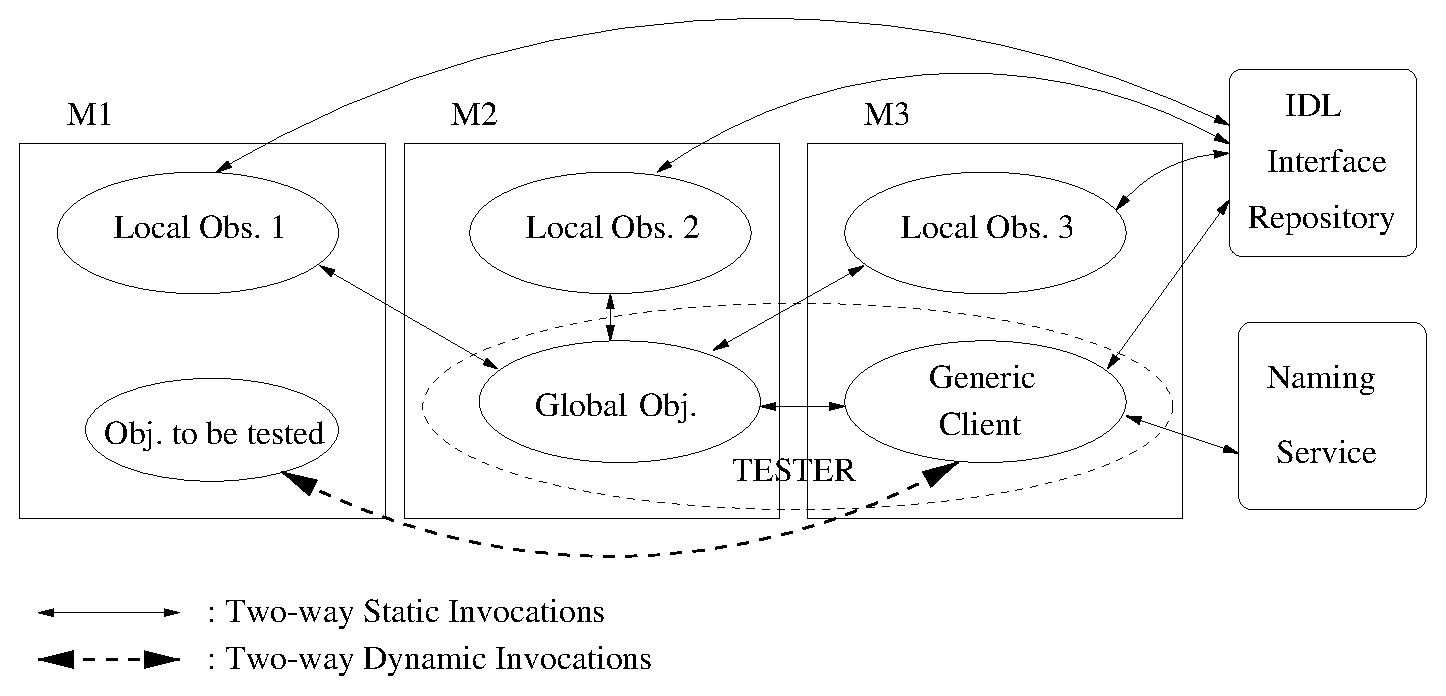
\includegraphics[width=8cm]{new_test_arch.eps}}
%\epsfxsize=11cm
%\epsfbox{test_arch.eps}
\caption{Tester architecture}
\protect\label{test_archi}
%\end{center}
\end{figure}

With the distribution constraint, we have to define a two-level
architecture for our observer. At the first stage we have one local
observer per workstation and at the second stage a global observer
which can be located at any site. Local observers and the global
observer has to cooperate in order to construct the global history of
invocations (this collaboration process is simplified because all the
invocations are synchronous). We have chosen CORBA as the distributed
infrastructure among the observers. The global observer interacts with
the tester using a CORBA IDL interface (so they may be located on
different sites). Interactions between the global observer and local
observers also use a CORBA IDL interface (in both directions). 


A local observer observes the local IIOP traffic and extracts useful
information from the segments
(name of the invoked operation, name of the target CORBA object
and value of the arguments, if any). The problem here is that IIOP
is a transport protocol and that we have to interpret the content of
the segment in order to extract the information we need. This
interpretation process uses the CORBA naming service to extract the
information about the target object and the interface repository to
extract the information about the invoked operation.\\
%Using the code generator of the ObjectGeode CASE from Verilog we have
%produced, from the SDL specification of the audio-conference service,
%an implementation in C language. We have focused on one component of
%this service which is the conference bridge process (it allows the
%reservation of a conference point terminal). In order to test
%completely this component using our testing platform, we have tried to
%encapsulate the generated code for this process in a CORBA server. To
%do this we have used a prototype developed by SEMA Group in an
%European project called SCREEN but without success. The CORBA
%encapsulation has to be done manually nd at this time we can not yet
%obtain the results of the execution of he test sequences generated by
%our platform.






\section{Conclusion}

We have shown that it is possible to obtain good bounds on the
minimum, maximum and average number of comparisons of merge sort
without resorting to advanced real analysis, like Fourier analysis,
nor complex analysis, like Mellin transforms. Whilst these powerful
techniques indeed bring the best results, they are not suitable for
postgraduate students in informatics who are introduced to sorting
algorithms.

Bachmann's \(O\)~notation is often misused for lower bounds and it is
deceptively simple because it must be abused to be really useful and
it seems to conflict with algebra over numbers. Using the
\(\Theta\)~notation when possible is better, but the extra work of
doing so then may become on par with determining asymptotic
equivalences, where multiplicative constants are explicit. It is
probably an overkill for most students to find out the exact linear
coefficients, but, for the most motivated, this paper shows how to do
so at the cost of slightly less precision sometimes.

\nocite{*}

\bibliographystyle{latex8}
\bibliography{iscc}

%\begin{figure}[htbp]
\begin{center}
\begin{bigbox}
\epsfig{file=msc_final.ps, width=10cm}
\end{bigbox}
\caption{Simplified test sequence of the conference-bridge module.}
\label{msc}
\end{center}
\end{figure}

Figure~\ref{msc} is the simplified MSC for the test sequence obtained
for the module representing the bridge-conference terminal. This
sequence brings to light all the interactions of this module (it
indeed covers all the transitions). We only show here the signal
exchanges between the two peers, i.e. the switch (SSF) and the user,
with which the bridge interacts. The environment here is schematized
by the frame of the figure. The scenarios that can be found in the
signal exchanges of the figure~\ref{msc} are the following:

\begin{itemize}
  \item the user 2 asks for a connection to the \audio by dialing
        number '083600001'. At the conference level, this is
        translated into the signal input \textsf{setupreq}. The
        conference module sends an \textsf{offhook} signal to the
        switch. This latter, after a chaining of exchanges with the PCS
        and a series of component activations, sends a
        \textsf{setupresp} signal which means that the communication
        can be established. First, the user receives a waiting
        message and, as soon as the communication is established, a
        welcome message. Once this latter is received, the user
        decides to on-hook: this sends a \textsf{releaseind} signal to
        the switch; this latter relays it to the conference module by
        means of the \textsf{releasereq}. This latter module
        acknowledges the disconnection request by the
        \textsf{releaseind} signal; then it receives a
        \textsf{line\_free} message, which indicates that the line is
        free again;

  \item the second part of the figure brings to the fore the following
        scenario: the user 1 calls the bridge, he receives the
        waiting signal and then the conference is opened; the waiting
        subscribers receive the welcome message; consequently the
        communication is established, they can talk to each other:
        this exchange is revealed by the reception of a
        \textsf{msg\_term} signal.
\end{itemize}

%We also supply the reader with a part of the TTCN  we got (see
%figure~\ref{ttcnseq}). The computed sequence corresponds to a
%black-box testing configuration, where the points of control and
%observation are located at the system level. Thus the exchanges
%between the environment and the user's block are visible.
%
%\begin{figure*}[!htbp]
%\begin{center}
%\begin{tabular}{l l}
%{\sf Test Case Name} &{\sf: network\_RI\_0}\\
%{\sf Group} &{\sf: network\_RI/}\\
%{\sf Purpose} &{\sf:}\\
%{\sf Default} &{\sf: DEF\_0}\\
%{\sf Comments} &{\sf: Generated by test oriented simulation of the test} \\
%&{\sf \- purpose network\_RI.msc}\\
%\end{tabular}
%\newline
%\scriptsize{
%\begin{tabular}{|p{5mm}|p{75mm}|p{15mm}|p{7mm}|}
%\hline
%{\sf Nr} &{\sf Behaviour Description} & {\sf Constraints Ref}&Verdict\\
%\hline
%{\sf 1} &{\sf env2users !offhook output} &&\\
%{\sf 2} &{\sf \hspace{0.1in}env2users !dial START TAC} & {\sf dial}&\\
%{\sf 3} &{\sf \hspace{0.2in}users ?msg CANCEL TAC} & {\sf msg\_3}&\\ 
%{\sf 4} &{\sf \hspace{0.3in}env2users !dial} & {\sf dial\_4}&\\
%{\sf 5} &{\sf \hspace{0.4in}env2users !releaseind} &&\\
%{\sf 6} &{\sf \hspace{0.5in}env2users !offhook} &&\\
%{\sf 7} &{\sf \hspace{0.6in}env2users !dial START TAC} & {\sf dial\_2}&\\
%{\sf 8} &{\sf \hspace{0.7in}env2users ?msg CANCEL TAC} & {\sf msg\_3}&\\
%{\sf 9} &{\sf \hspace{0.8in}env2users !dial} & {\sf dial\_4}&\\
%{\sf 10} &{\sf \hspace{0.9in}env2users !talk} & {\sf talk\_6}&\\
%{\sf 11} &{\sf \hspace{1.0in}env2users !offhook} &&\\
%{\sf 12} &{\sf \hspace{1.1in}env2users !dial START TAC} & {\sf dial\_7}&\\
%{\sf 13} &{\sf \hspace{1.2in}env2users ?msg CANCEL TAC} & {\sf msg\_3}&\\
%{\sf 14} &{\sf \hspace{1.3in}env2users !dial START} & {\sf dial\_7}&\\
%{\sf 15} &{\sf \hspace{1.4in}env2users ?msg CANCEL} & {\sf msg\_3}&(P)\\
%{\sf 16} &{\sf \hspace{1.4in} ? TIMEOUT TAC} &&F\\
%{\sf 17} &{\sf \hspace{1.2in} ? TIMEOUT TAC} &&F\\
%{\sf 18} &{\sf \hspace{0.6in} ? TIMEOUT TAC} &&F\\
%{\sf 19} &{\sf \hspace{0.1in} ? TIMEOUT TAC} &&F\\
%\hline
%\end{tabular}
%}
%\caption{TTCN sequence}
%\label{ttcnseq}
%\end{center}
%\end{figure*}


\end{document}
